% This template has been tested with LLNCS DOCUMENT CLASS -- version 2.20 (24-JUN-2015)

%"runningheads" enables:
%  - page number on page 2 onwards
%  - title/authors on even/odd pages
%This is good for other readers to enable proper archiving among other papers and pointing to
%content. Even if the title page states the title, when printed and stored in a folder, when
%blindly opening the folder, one could hit not the title page, but an arbitrary page. Therefore,
%it is good to have title printed on the pages, too.
\documentclass[runningheads,a4paper]{llncs}[2015/06/24]

%cmap has to be loaded before any font package (such as cfr-lm)
\usepackage{cmap}
\usepackage[T1]{fontenc}

\usepackage{graphicx}

%some custom math stuff
\usepackage{amsmath}
\usepackage{amssymb}

% für neue deutsche Rechtschreibung
\usepackage[english,ngerman]{babel}

% für englische Rechtschreibung
%Even though `american`, `english` and `USenglish` are synonyms for babel package (according to https://tex.stackexchange.com/questions/12775/babel-english-american-usenglish), the llncs document class is prepared to avoid the overriding of certain names (such as "Abstract." -> "Abstract" or "Fig." -> "Figure") when using `english`, but not when using the other 2.
%english has to go last to set it as default language
%\usepackage[ngerman,english]{babel}

%Eingabeformat UTF-8
\usepackage[utf8]{inputenc}

%Hint by http://tex.stackexchange.com/a/321066/9075 -> enable "= as dashes
\addto\extrasenglish{\languageshorthands{ngerman}\useshorthands{"}}

%cfr-lm is preferred over lmodern. Reasoning at http://tex.stackexchange.com/a/247543/9075
\usepackage[%
rm={oldstyle=false,proportional=true},%
sf={oldstyle=false,proportional=true},%
tt={oldstyle=false,proportional=true,variable=true},%
qt=false%
]{cfr-lm}
%
%if more space is needed, exchange cfr-lm by mathptmx

\graphicspath{{graphics/}}

%Tweaks by IPVS/AS
\usepackage{lncs_as}

%for demonstration purposes only
\usepackage[math]{blindtext}

%Sorts the citations in the brackets
%It also allows \cite{refa, refb}. Otherwise, the document does not compile.
%  Error message: "White space in argument"
\usepackage{cite}


%% If you need packages for other papers,
%% START COPYING HERE
%% COPY ALSO cmap and fontenc from lines 10 to 12

%extended enumerate, such as \begin{compactenum}
\usepackage{paralist}

%put figures inside a text
%\usepackage{picins}
%use
%\piccaptioninside
%\piccaption{...}
%\parpic[r]{\includegraphics ...}
%Text...

%for easy quotations: \enquote{text}
\usepackage{csquotes}

%enable margin kerning
\usepackage{microtype}

%tweak \url{...}
\usepackage{url}
%\urlstyle{same}
%improve wrapping of URLs - hint by http://tex.stackexchange.com/a/10419/9075
\makeatletter
\g@addto@macro{\UrlBreaks}{\UrlOrds}
\makeatother
%nicer // - solution by http://tex.stackexchange.com/a/98470/9075
%DO NOT ACTIVATE -> prevents line breaks
%\makeatletter
%\def\Url@twoslashes{\mathchar`\/\@ifnextchar/{\kern-.2em}{}}
%\g@addto@macro\UrlSpecials{\do\/{\Url@twoslashes}}
%\makeatother

%diagonal lines in a table - http://tex.stackexchange.com/questions/17745/diagonal-lines-in-table-cell
%slashbox is not available in texlive (due to licensing) and also gives bad results. This, we use diagbox
%\usepackage{diagbox}

%required for pdfcomment later
\usepackage[hyperref,svgnames]{xcolor}

\usepackage{listings}
\lstloadlanguages{java}
\lstset{language=java,numbers=left,captionpos=b}


%enable nice comments
%this also loads hyperref
\usepackage{pdfcomment}
%enable hyperref without colors and without bookmarks
\hypersetup{hidelinks,
   colorlinks=true,
   allcolors=black,
   pdfstartview=Fit,
   breaklinks=true}
%enables correct jumping to figures when referencing
\usepackage[all]{hypcap}

\newcommand{\commentontext}[2]{\colorbox{yellow!60}{#1}\pdfcomment[color={0.234 0.867 0.211},hoffset=-6pt,voffset=10pt,opacity=0.5]{#2}}
\newcommand{\commentatside}[1]{\pdfcomment[color={0.045 0.278 0.643},icon=Note]{#1}}

%compatibality with packages todo, easy-todo, todonotes
\newcommand{\todo}[1]{\commentatside{#1}}
%compatiblity with package fixmetodonotes
\newcommand{\TODO}[1]{\commentatside{#1}}

%enable \cref{...} and \Cref{...} instead of \ref: Type of reference included in the link

\usepackage[capitalise,nameinlink,ngerman]{cleveref}
%\usepackage[capitalise,nameinlink,english]{cleveref}
%Nice formats for \cref - only for English texts
%\crefname{section}{Sect.}{Sect.}
%\Crefname{section}{Section}{Sections}

\usepackage{xspace}
%\newcommand{\eg}{e.\,g.\xspace}
%\newcommand{\ie}{i.\,e.\xspace}
\newcommand{\eg}{e.\,g.,\ }
\newcommand{\ie}{i.\,e.,\ }

%introduce \powerset - hint by http://matheplanet.com/matheplanet/nuke/html/viewtopic.php?topic=136492&post_id=997377
\DeclareFontFamily{U}{MnSymbolC}{}
\DeclareSymbolFont{MnSyC}{U}{MnSymbolC}{m}{n}
\DeclareFontShape{U}{MnSymbolC}{m}{n}{
    <-6>  MnSymbolC5
   <6-7>  MnSymbolC6
   <7-8>  MnSymbolC7
   <8-9>  MnSymbolC8
   <9-10> MnSymbolC9
  <10-12> MnSymbolC10
  <12->   MnSymbolC12%
}{}
\DeclareMathSymbol{\powerset}{\mathord}{MnSyC}{180}

% correct bad hyphenation here
\hyphenation{op-tical net-works semi-conduc-tor}

%% END COPYING HERE


\begin{document}

\title{Feature-Extraktion für Sensordaten zur Maschinenüberwachung}
%If Title is too long, use \titlerunning
%\titlerunning{Short Title}

\author{Niklas Kleinhans}
5
\supervisor{Mathias Mormul}

\seminar{Advanced Topics in Data Management}

\semester{WS 2018/2019}

\abgabedatum{Stuttgart, 05.11.2018}

\institute{}

\frontpagede % creates the frontpage (in German)
%\frontpageen % creates the frontpage (in English)

\thispagestyle{empty}
\cleardoublepage

\maketitle


\begin{abstract}
  Maschinen werden bis zum kleinsten Bauteil immer intelligenter und ermöglichen es Daten unterschiedlicher Struktur und Komplexität in großen Mengen aufzunehmen. 
  Im industriellen Umfeld wird dabei von \enquote{Industrie 4.0} gesprochen. 
  Der Begriff ummantelt die Beschreibung einer neuen Industriegeneration, in der Systeme durch technologische Weiterentwicklungen intelligent werden und miteinander vernetzt sind. 
  Ein Ergebnis dieser Intelligenz ist die Maschinenüberwachen. 
  Die Maschinenen sollen mithilfe von Livedatenanalyse überwacht und dadurch der aktuellen oder auch zukünftige Maschinenzustand ermittelt werden. 
  Um diese Intelligenz zu erreichen werden unteranderem Sensordaten aufgenommen und anschließend zur Analyse weiterverarbeitet.
  Die dadurch entstehenden Datenbilder lassen sich oft nicht mehr durch einfache, beispielsweise lineare, Analysmodelle abbilden, was eine rechenintensieveren Analyse zur Folge hat.
  Die Anforderung an die Sensordatenanalyse im Maschinellenumfeld sind vorallem eine schnelle Datenverarbeitung mittels geringer Rechenkapazität.
  Um dies zu gewährleisten wird versucht die komplexen Sensordaten so aufzubereiten, dass diese weiterehin durch weniger komplexe Analyseverfahren verarbeitet werden können.
  In dieser Arbeit werden Verfahren vorgestellt die mithilfe von \enquote{Feature Extraktion} diese Anforderungen erfüllen.
  Dabei steht der Begriff \enquote{Feature} für ein Merkmal, wodurch sich Daten unterscheiden lassen.
  Diese werden extrahiert und bilden die Grundlage zur Datendifferenzierung. 
  Es werden die Herausforderungen in der Sensordatenanalyse, speziell in der Livedatenanalyse, beschrieben und Algorithmen vorgestellt.

\end{abstract}
\begin{keywords}
Maschinenüberwachung, Feature Extraktion, Maschinelles Lernen, Sensordaten, Livedaten, Livedatenanalyse
\end{keywords}

\section{Einleitung}

\begin{center}
  -TODO- Umlaute
\end{center}

%Ein großer Bereich der vierten Industriegeneration ist das \enquote{Internet der Dinge} oder im Englischen \enquote{Internet of Things (IoT)}. 
%Darunter versteht man ein erweitertes Konzept des aktuel bestehenden Internets. 
%Es findet nicht mehr nur ein reiner Daten-/Informationsaustausch mittels unterschiedlicher Medientypen statt, sondern große Systeme bis hin zu kleinsten Komponenten werden Vernetzt und bilde eine Kommunikationsschicht~\cite{Jaspindustrie}.
%Durch diese Kommunikation entstehen Datenflüsse die einerseits in großen Rechenzentren gespeichert werden können und andererseits bieten sie eine Grundlage zur Livedatenanalyse.

Maschinen bestehen oft aus mehreren Komponenten und sind anschließend Teil eines großen Systems.
Um zu gewährleisten, dass das System korrekt funktioniert und auch möglichst selten ausfällt, werden Daten über Controllersysteme und Sensoren jeder einzelnen Komponente aufgenommen.
In einem großen System fallen durch kontinuierliche Datenaufnahme große Datenmengen an.
Um schon preventiv Maschinenausfälle zu vermeiden werden diese Daten oft an Überwachungssysteme übertragen um anschließend mithilfe von Schwellwertüberschreitungen den Systemzustand darzustellen.
Diese Datenbilder werden in Form von Diagrammen, Ampelsystemen, oder ähnlichem visualisiert und für den Menschen lesbar dargestellt.
Es ist die Rede von \enquote{Condition-Monitoring}.

Um noch mehr Informationen aus diesen Daten zu erhalten werden unterschiedliche Analyseverfahren angewendet um Anomalien festzustellen und auf diese anschließend zu reagieren.
Die Herausforderung dabei ist der kontinuierliche Datenfluss.
Die Daten müssen, ähnlich zur Livedatenanalyse, direkt verarbeitet werden.
Schwellwertüberschreitungen können diese Livedaten leicht verarbeiten, da jeweils nur ein Datenpunkt betrachtet werden muss.
Nähere Zusammenhänge innerhalb eines Datenpakets oder sogar zwischen mehrere Datenpaketen zu erkennen ist Rechenaufwändiger.
Betrachten man mehere Daten innerhalb eines Zeitfensters können diese Datenpunkte mittels Approximationen wie in Abbilding\ \ref{fig:FFETimeSeries} (a), (b) und (c) verglichen werden. 
Die Zeitreihendaten sehen in diesem Fall für Menschen nahezu gleich aus. 
Dennoch kann durch Anwenden von Analysverfahren ein gewisser Unterschied erkannt werden.
In Abbildung\ \ref{fig:FFETimeSeries} (d), wurden die Zeitreihen in einem Merkmalsraum, im englischen \enquote{Feature Space}, dargestellt. 
Zeireihe (a) und (c) sind weiterhin sehr ähnlich.
Zeireihe (b) unterscheidet sich etwas im Vergleich zu (a) und (c).

\begin{figure}
  \centering
  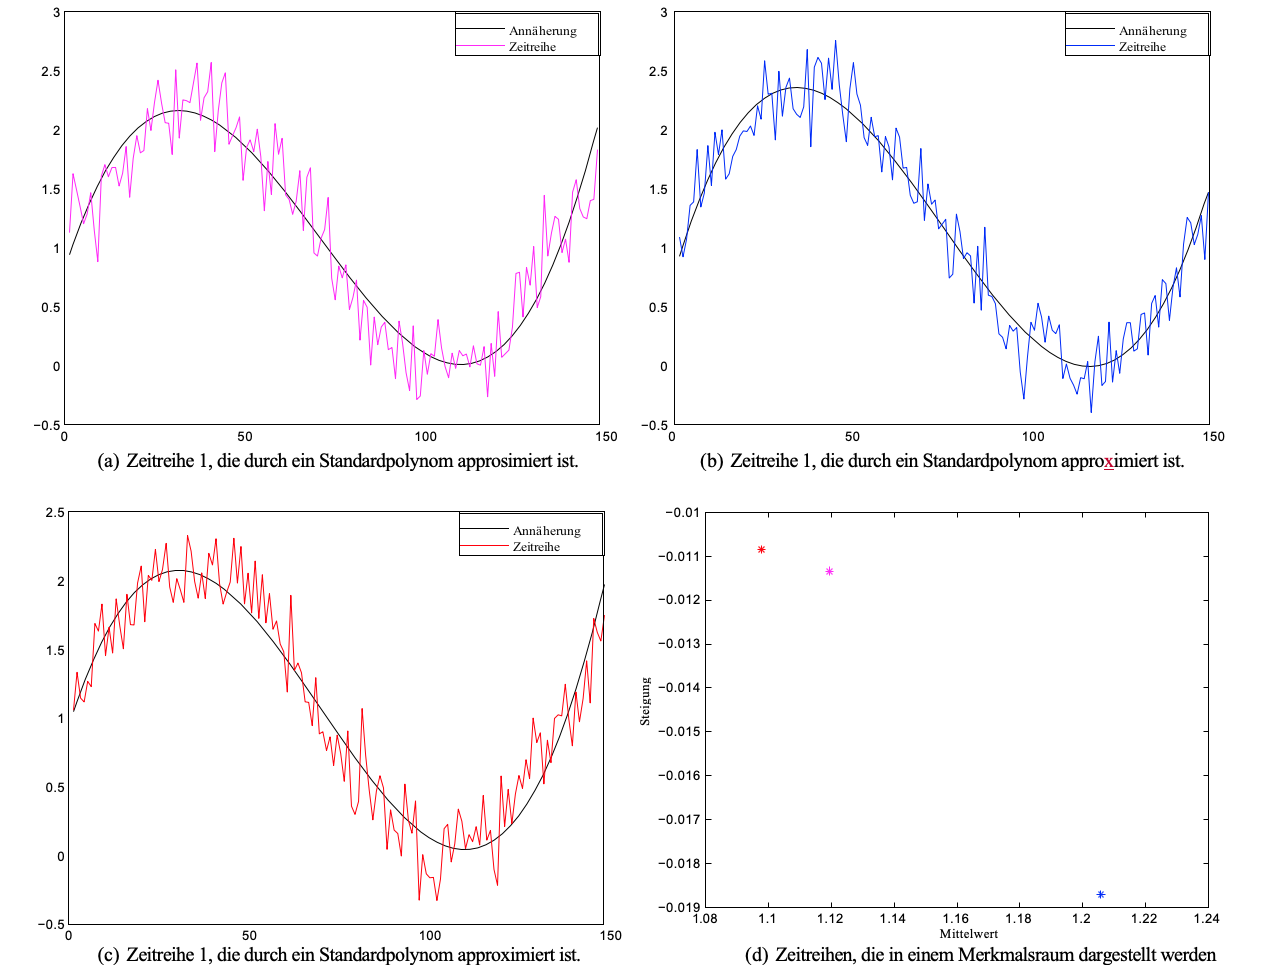
\includegraphics[width=1\textwidth]{FastFeatureExtractionTimeSeries.png}
  \caption{Drei standard ploynom Approximationen mittes least-squared. Die Drei Approximationen werden in Abbildung (d) in einem Merkmalsraum dargestellt~\cite{gensler2015fast}.}
  \label{fig:FFETimeSeries}
\end{figure}


Dieser Merkmalsraum wird durch das Analysieren der Daten auf gewissen Merkmale, im englischen \enquote{Features}, erstellt.
Der Merkmalsraum bietet eine weitere Möglichkeit Datenmiteinander zu vergleichen, Anomalien zu erkennen oder die Daten zu klassifizieren. 
Um solche Verfahren anwenden zu können müssen diese Merkmale zuvor extrahiert werden. 
Es ist die Rede von \enquote{Feature Extraktion}.

In diesem Fall handelt es sich um eine polynomielle Approximation der Zeitreihendaten. 
Diese muss in in jedem Zeitschritt für den gewählt Zeitraum neu berechnet werden. 
Dies kann je nach Dimension des Polynoms sehr Rechenaufwändig und komplex werden.
Bei einer hohen Abtastrate und einer großen Anzahl an Sensoren entstehen rießige Datenmengen unter harten Laufzeitbedingungen analysiert werden müssen.
Ein weiterer Vorteil der \enquote{Feature Extraktion} ist das Reduzieren der koplexität dder Daten. Die Daten müssen nicht mehr selbst über polynomielle Modelle analysiert werden, sondern die extrahierten Merkmalen können als Eingabe für die Analyseverfahren dienen. Somit können komplexe polynomielle Datenbilder mithilfe von beispielsweise linearer Verfahren analysiert werden.

In dieser Arbeit wird zu Beginn in Kapitel \ref{kap:grundlagen} die grundlegende Struktur von Sensordaten beschrieben, der Zusammenhang mit Livedaten diskutiert und anschließend die damit verbundene Verwendung von \enquote{Feature Extraktions Verfahren} besprochen. 
In Kapitel \ref{kap:featureextraktion} werden die Randbedingungen und Herausforderungen an Algorithmen zur kontinuierlichen Livedatenanalyse besprochen und Ansatze sowie Algorithmen vorgestellt, die sich mit desem Probelmen auseinander setzen.
\section{Verwandte Arbeiten}
Viele Arbeiten  beschäftigen sich damit Sensordaten mit Hilfe von analytischen Methoden zu verarbeiten. 
Ein Beispiel ist die Arbeit \enquote{Using Machine Learning on Sensor Data} von Alexandra Moraru et al.~\cite{moraru2010using}. 
In dieser wird die Anzahl von Mitarbeitern im Büro anhand von Sensordaten vorhergesagt.
Dabei werden klassische Klassifikations- und Regressionsverfahren angewendet und validiert. 
Die Verfahren werden auf einen Trainingsdatensatz trainiert und anschließend auf weitere Datenpakete angewendet. 
Dabei wurden die Merkmale, an welchen die Anzahl der Mitarbeiter vorhergesagt werden sollen vordefiniert. 

Bei komplexeren Problemen, wie bei der Maschinenüberwachung, müssen die Merkmale oft erst gefunden werden. 
Diese Merkmale können neben einfachen Schwellwertüberschreitungen auch beispielsweise gewisse Datenmuster sein. 
Diese  Andre Gensler, Thiemo Gruber und Bernhard Sick beschreiben Verfahren in ihrer Arbeit \enquote{Fast Feature Extraction For Time Series Analysis Using Least-Squares Approximations with Orthogonals Basis Functions}, mit welchen sie diese Merkmale, unter harter Laufzeit und Speicheranforderungen, erkennen. 

Die Analyseverfahren benötigen oft sehr viel Rechenleistung da die Proleme, welche einer nicht linearen Komplexität entsprechen, sehr aufwändig zu Berechnen sind. 
Man spricht dabei von Höherdimensionalen Problemen. 
Fabian Mörchen beschreibt in seiner Arbeit \enquote{Time series feature extraction for data mining using DWT and DFT} eine Methode um die Dimension von Zeitreihendaten zu reduzieren. 
Er Optimiert dabei die Auswahl der Koeffizienten und reduziert damit den Berechnungsaufwand für Analyseverfahren.

\begin{center}
  -TODO- Die weiteren Referenzen zusammenfassen
\end{center}

\section{Grundlagen}\label{kap:grundlagen}
Sensordaten haben gewissen Eigenschaften die dazu führen, dass diese vor der Analyse vorverarbeitet werden müssen, um eine effiziente Anwendung von Algorithmen gewährleisten zu können. 
In diesem Kapitel sollen diese Eigenschaften diskutiert und anschließend einige Grundlagen für die in Kapitel \ref{kap:featureextraktion} diskutierten Algorithmen zur Analyse von Sensordaten besprochen werden.
\subsection{Was sind Sensordaten}\label{kap:sensordaten}

Um den Ablauf einer Maschine zu koordinieren und den aktuellen Zustand zu Überwachen werden oft Sensoren an den Maschinen angebracht. 
Diese Daten werden zu definierten Taktzeiten aufgenommen und weiterverarbeitet. 
Es kann sich dabei um einfache Kontaktsensoren handeln, mit einer begrenzten Anzahl an Zuständen oder um Sensoren mit einem reellen Zustandsbereich, wie Umgebungssensoren (Luftdruck-, Temperatursensor, etc.). 
In Abbildung\ \ref{fig:datasetoffice} sind Sensordaten in Form eines Datenplots dargestellt. 
Es handelt sich um Licht-, Temperatur- und Luftfeuchtigkeitssensordaten aus einem Büro im Zeitraum eines Arbeitstages. 
Abgebildet sind die Sensordaten zwischen $6:00$ Uhr und $19:00$Uhr.
\begin{figure}
    \centering
    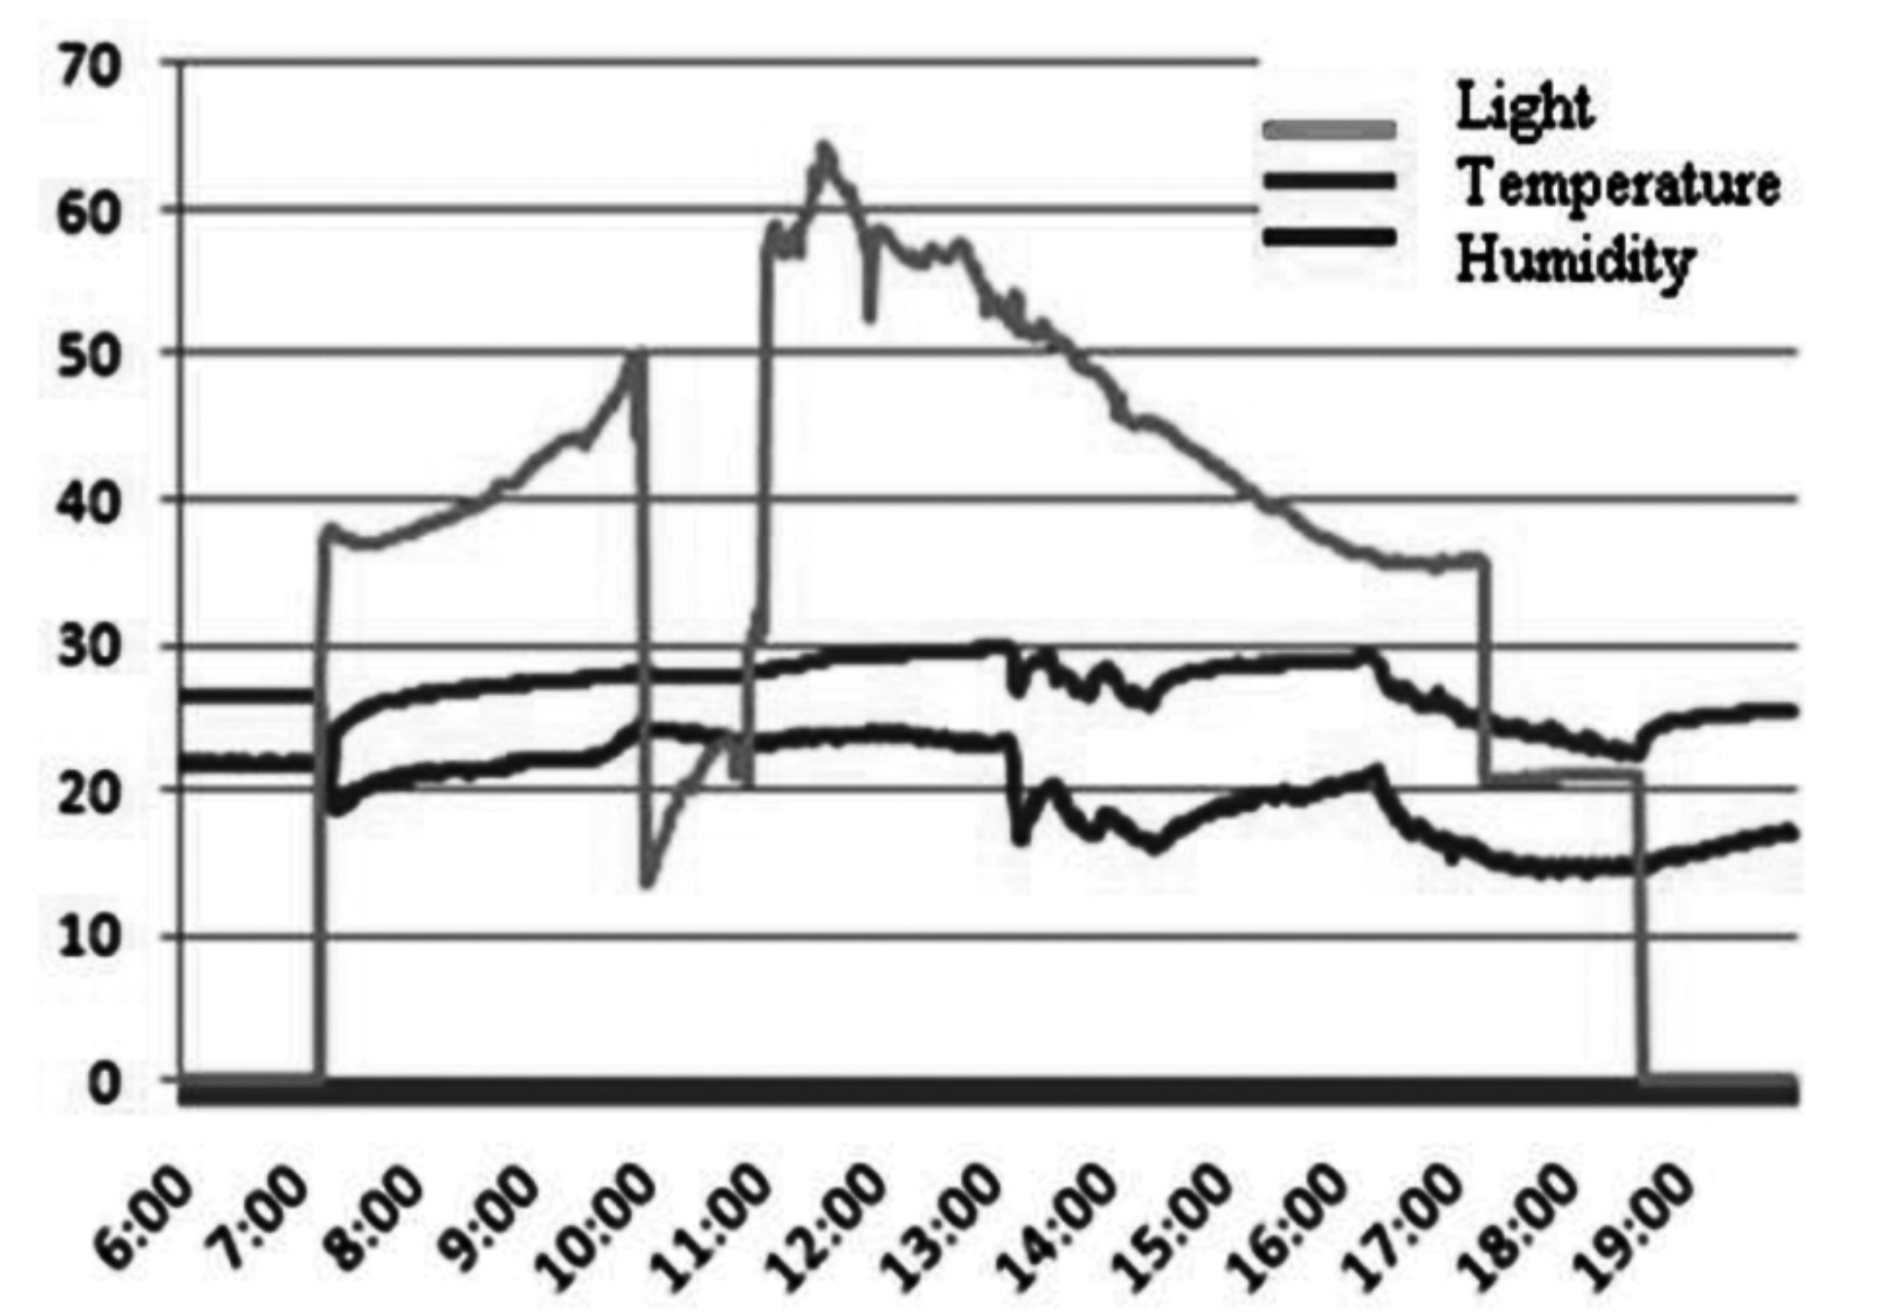
\includegraphics[width=.8\textwidth]{datasetOffice.png}
    \caption{Abweichung der Sensordaten anhand von Licht, Temperatur und Luftfeuchtigkeit im Büro innerhalb von einem Arbeitstag~\cite{moraru2010using}}
    \label{fig:datasetoffice}
\end{figure}

In der Arbeit \enquote{Using machine learning on sensor data} von Alexandra Moraru et al. ~\cite{moraru2010using} wurde durch Aufnahme dieser Daten ein datengetriebenes Model entwickelt, welches erkennen kann, wieviele Personen sich zu einem Zeitpunkt im Büro befinden.

Um solche Sensordaten zu verarbeiten müssen diese in eine mathematische Struktur gebracht werden. 
Dazu werden Zeitpunkte aus den Datensätzen gewählt und in einem Vektor dargestellt.
Ein Datensatz zum Zeitpunkt $6:00$ Uhr mit den Werten Licht = $0$, Temperatur=$22$ und Luftfeuchtigkeit = $25$ könnte dargestellt werden als:
\begin{equation}
    x_1 =
  \begin{pmatrix}
      0\\
      22\\
      25
  \end{pmatrix}
  \in \mathbb{R}^D
\end{equation}
Ein Vektor enthält somit einen Sensordatensatz zu einem Aufnahmezeitpunkt. Um Zeiträume darzustellen werden die Daten in eine Matrixform gebracht. Beispielsweise erhält man bei einer stündlichen Abtastrate und einem Zeitraum von $8:00$ Uhr bis $17:00$Uhr folgende Matrix:
\begin{equation}
    x_{1,10}
    \begin{pmatrix}
       38 & 40 & 46 & 24 & 60 & 58 & 51 & 44 & 40 & 36\\
       20 & 22 & 22 & 24 & 24 & 24 & 20 & 18 & 20 & 17\\
       25 & 28 & 28 & 28 & 29 & 30 & 20 & 27 & 29 & 26
    \end{pmatrix}
    \in \mathbb{R}^{D \times N}
\end{equation}

Diese mathematische Darstellung ist nur ein Beispiel und kann beliebig strukturiert werden.
Die erzeugte Matrix kann anschließend als Eingabe für Analysealgorithmen dienen.
Schon bei diesen geringen Datenmengen entsteht eine $D \times N $ große Matrix mit: 
\begin{itemize}
  \item $D=$ Anzahl der Parameter (Sensoren)
  \item $N=$ Anzahl der Daten.
\end{itemize}

Sollen auch noch Daten Raumübergreifend analysiert werden, können diese in Form eines Tensors dargestellt werden. Bei $M$ vielen Räumen entsteht ein $D \times N \times M$ großer Tensor.
Schon anhand dieses simplen Beispiels wird die Datenmenge und Komplexität der Daten ersichtlich.
In der Maschinenüberwachung entstehen dadurch schnell Datensätze im Millionenbereichen und da jede Komponente einer Maschine oft mit mehreren Sensoren ausgestattet ist, entstehen riesige Tensoren.

Neben klassischen Regressionsverfahren zur Datenanalyse, welche oft für Anomaliedetektionen verwendet werden, gibt es auch verschiedene Klassifikationsverfahren. Dazu werden den Datensätzen manuell oder automatisiert Klassen hinzugefügt, welche jedem aufgenommenen Datenvektor eine Klasse zuordnet.

Mathematisch dargestellt erhalten wir dann einen Datensatz zum Zeitpunkt $t_1$ in Form eines Tupels $\tau_1=(t_1,x_1)$. Die für den Zeitpunkt definierten Merkmale sind dann in $x_k$ mit $(k=1_d)$ und $d \in D$. Diesem Tupel wird abhängig von den verwendeten Verfahren eine Klasse $y_1$ zugewiesen~\cite{gay2013feature}. Für den Zeitraum $(t_1,...,t_n)$ mit $n \in \mathbb{N}$ vielen Daten erhalten wir den Datensatz 
\begin{equation}
  K=\{ (\tau_{1_d},y_{1}), ... , (\tau_{n_d},y_n) \}
  \label{equ:trainingset}
\end{equation}
Das Ziel kann es sein das Tupel $(t_{n+1},y_{n+1})$ vorherzusagen.

Es werden auch nicht nur feste Zeiträume betrachtet. 
Durch dauerhaft laufende Maschinen entstehen kontinuierliche Datenströme.
Daraus folgt ein kontinuierlich wachsender Datenbestand.
Um ressourcenschonend und möglichst in Echtzeit die Daten zu analysieren, werden harte Speicher- und Laufzeitbedinungen an Analysealgorithmen gestellt.

Ein großer Vorteil der Sensordaten ist die starke Korrelation zwischen den Daten. Eine zum Zeitpunkt $t$ aufgenommener Datensatz enthält oftmals ähnliche Informationen wie vor $t$ aufgenommenen Datensätze. Durch diese Eigenschaft, können Daten schon oft im Voraus stark reduziert werden~\cite{morchen2003time}.
Die Korrelation führt zusätzlich noch zu einer weiteren Informationsquelle, weshalb Sensordaten meist auch als Zeitreihendaten analysiert werden.
Diese Analyse berücksichtigt nicht nur einzelne Datenpunkte, sondern setzt sie Zeitlich Verbindung.



\subsection{Feature Extraktion}\label{kap:featureextraktionuebersicht}
Im maschinellen Lernen werden im Wesentlichen zwei Methoden zur Datenanalyse betrachtet. Bei der \textbf{Regression} werden die Eingabedaten auf Datenwerte reduziert ähnlich zur Approximation in Abbildung\ \ref{fig:FFETimeSeries}. Zu dem Datensatz aus den Sensordaten eines Büroalltags in Kapitel\ \ref{kap:sensordaten} könnte mithilfe von Regression die Anzahl an Mitarbeitern im Büro berechnet werden. In der \textbf{Klassifikation} werden Daten bestimmten Klassen zugeordnet. Im Gegensatz zur Regression würden nicht die Anzahl der Mitarbeiter, sondern Beispielsweise die Klassen \enquote{Büro besetzt} und \enquote{Büro unbesetzt} ausgegeben werden.

In beiden Verfahren ist die Grundlage der Entscheidung die Dateneingabe und die dazu gehörigen Parameter. Somit ist die Einhaltung der Algorithmenschranken (Speicher- und Laufzeitbedingungen) abhängig von den Parametern $D$. Es gibt unterschiedliche Gründe, weshalb versucht wird die Anzahl der Eingabeparameter anzupassen~\cite{alpaydin2014introduction}:
\begin{itemize}
  \setlength{\itemsep}{3pt}
  \renewcommand\labelitemi{\textbullet}
  \item Die Komplexität eines Lernalgorithmus hängt von der Anzahl an Eingabe Dimensionen $D$ und der Anzahl der Daten $N$ ab. Wird die Anzahl an Dimensionen und somit Parametern reduziert, dann reduziert sich auch die Komplexität.
  \item Wenn die richtigen Parameter ausgewählt werden, sind die Algorithmen teilweise sogar stabiler~\cite{morchen2003time}
  \item Wenn eine Eingabe keinen Einfluss auf die Funktion und das Ergebnis des Algorithmus hat, können diese Kosten eingespart werden.
  \item Modelle aus Lernalgorithmen sind oft auf kleine Datensätze robuster, da diese eine geringere Varianz und Rauschen aufweisen.
  \item Wenn Daten durch weniger Merkmale beschrieben werden können, bekommt der Mensch ein besseres Verständnis über den gesamten Prozess.
  \item Je weniger Dimensionen, desto leichter die Visualisierung.
\end{itemize}

Aus diesen Gründen wird versucht die Anzahl der Eingabeparameter in einen Algorithmus möglichst zu reduzieren. Um so eine Dimensionsreduktion zu erreichen gibt es zwei Hauptansätze:
\paragraph{Feature Selektion} ist ein Ansatz, indem die Dimension $D$ auf eine Dimension $L$ reduziert wird. Dabei werden interessante Parameter aus der Parametermenge entnommen und die restlichen $D-L$ Parameter werden verworfen.
In Abbildung \ \ref{fig:featureselection} ist ein tabellarisches Beispiel zu sehen, an dem nur relevante Parameter ausgewählt werden.
\enquote{Features} sind dabei Merkmale, wodurch sich Daten unterscheiden lassen. In diesem Ansatz sind die Merkmale direkt die ausgewählten Eingabeparameter~\cite{alpaydin2014introduction}.

\begin{figure}
  \centering
  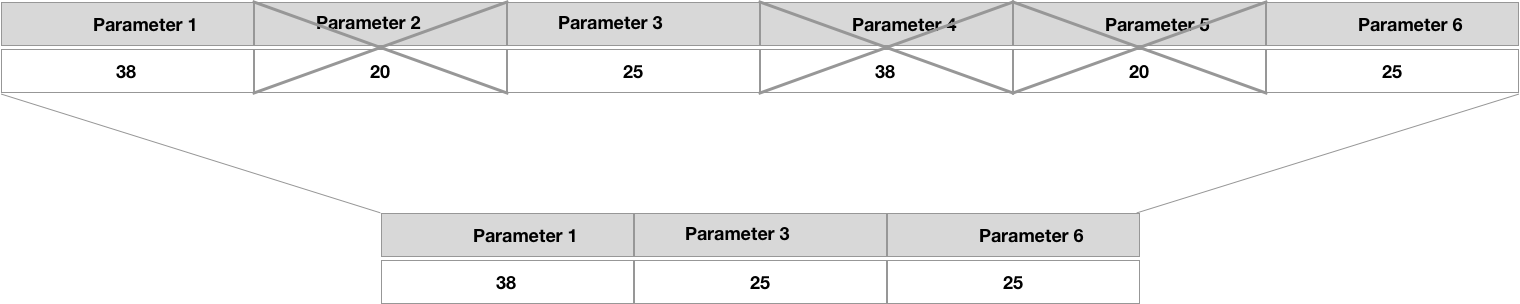
\includegraphics[width=.8\textwidth]{featureselection.png}
  \caption{Feature Selektion anhand eines Tabellenbeispiels. Es werden nur relevante Parameter ausgewählt.}
  \label{fig:featureselection}
\end{figure}


\paragraph{Feature Extraktion} dagegen entnimmt nicht vorhandene Eingabeparameter sondern geniert bzw. extrahiert aus den vorhandenen Parameter neue Merkmale. Die Anzahl an Merkmalen ergibt die neue Dimension $L$ ~\cite{alpaydin2014introduction}.
Merkmale können einfache, auf die Parameter angewedete, Funktionen sein, wie in Abbildung\ \ref{fig:FFETimeSeries} der Durchschnitt und die Steigung im Merkmalsraum (d). Oder komplexere Parameterkombinationen in höher Dimensionalenräumen, wie Verlaufsmuster von Raumflächen.

\begin{figure}
  \centering
  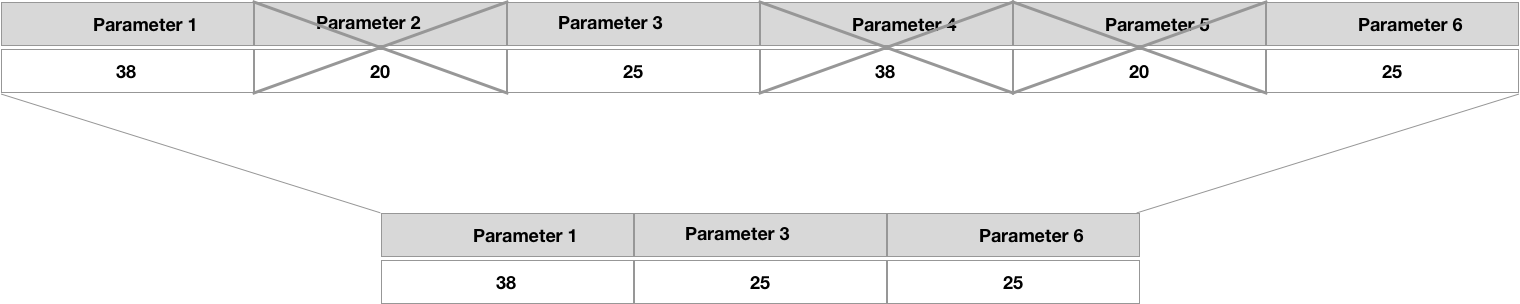
\includegraphics[width=.8\textwidth]{featureextraction.png}
  \caption{Feature Extraktion anhand eines Tabellenbeispiels. Es werden aus den bisherigen Parametern neue Parameter erstellt.}
  \label{fig:featureextraktion}
\end{figure}

Auf Lernalgorithmen angewendet ist es letztlich immer das Ziel die Features so zu wählen und zu parametrisieren, dass der ermittelte Wert oder die ermittelten Zuordnung aus einem Lernalgorithmus dem tatsächlichen möglichst ähneln. Formal beschrieben anhand dem Datensatz \ref{equ:trainingset}. Sei $p(x_i)$ die Funktion, welche das Ergebnis des gewählten Algorithmus und des Trainingsdatensatzes ist. Es soll versucht werden den Fehlerunterschied

\begin{equation}
  \sigma = p(x_i)-y_i
\end{equation}

möglichst zu reduzieren~\cite{gensler2015fast}. Die konkreten Herausforderungen und Herangehensweisen in der Maschinenüberwachung werden in dem folgenden Kapitel besprochen.

\section{Feature Extraktion bei kontinuierlichen Livedaten}\label{kap:featureextraktion}

Durch die stetige Aufnahme von Sensordaten um Maschinen zu überwachen, entsteht ein kontinuierlicher Datenfluss. 
Wie in den vorherigen Kaptiteln beschrieben, stellt diese Eigenschaft eine hohe Anforderung an Lernalgorithmen. 
Einige Lernalgorithmen verwenden das Konzept des \enquote{Lazy Learnings}, im Deutschen \enquote{träges Lernen}. 
Bei diesen Lernalgorithmen wird das Modell auf Anfrage erstellt. 
Das bedeutet, jede Eingabe startet eine neue Modellbildung und fordert daher in kürzester Zeit eine hohe Rechenleistungen. Beim \enquote{Eeager Learning}, im Deutschen \enquote{Eifriges Lernen}, hingegen wird schon im Vorfeld mithilfe von Trainingsdaten ein Model bereitgestellt. 
Der Ressourcenverbrauch bei einer Anfrage von neuen Daten ist dann sehr gering~\cite{Gay2013}. 

Bei den kontinuierlichen Livedaten in der Maschinenüberwachung stehen die Daten meist auch zeitlich in Korrelation. Daher ist die Rede von Zeitreihendaten. Die Reihenfolge dieser Daten spielt bei der Analyse eine große Rolle. Zeitreihendatensätze werden mathematisch wie in dem Datensatz \ref{equ:trainingset} dargestellt. Eines der Ziele für Lernalgorithmen kann es sein aus dem Datensatz \ref{equ:trainingset} die Daten 

\begin{equation}
  \tau_{n+1}, \tau_{n+2}, ...
  \label{equ:predictionset}
\end{equation}
vorherzusagen.

Das Ziel ist es aus den Daten mittels Analysealgorithmen Informationen über die Maschine zu gewinnen. 
Um dies effizient zu erreichen, können gewissen Merkmale vordefiniert oder extrahiert werden. 
Eine bewerte Methode ist das Zerlegen der Zeitreihendaten.

\subsection{Zeitreihenzerlegung}
Bei der Zeitreihenzerlegung werden die zeitlich korrelierenden Daten durch additive oder multiplikative Verfahren in Merkmale zerlegt. 
Diese können anschließend wieder durch zusammenführen in den Grunddatensatz zurückgeführt werden.
Die zerlegten Datensätze liefern im zerlegten Zustand jeweils eine spezielle Information, basierend auf der Art der Zerlegung.

\subsubsection{Zerlegung in Trend und Saisonkomponente}
Bei der Zerlegung von Zeitreihen in Trend- und Saisonkomponenten wird die Zeitreihe typischerweise in folgende Komponenten aufgeteilt~\cite{Leonard2018}:
\begin{itemize}
  \item $T_t$ Trendkomponente, stellt den langfristigen Verlauf dar.
  \item $C_t$ Zykluskomponente, stellt wiederholte Schwankungen dar.
  \item $S_t$ Saisonkomponente, stellt Schwankungen in festen und bekannten Zeiträumen dar.
  \item $I_t$ unregelmäßige Komponente, stellt unregelmäßige Schwankungen dar.
\end{itemize}
Dabei werden Trend- und Zykluskomponenten gerne zu einer Trendzykluskomponente zusammengefasst.



\begin{figure}
  \centering
  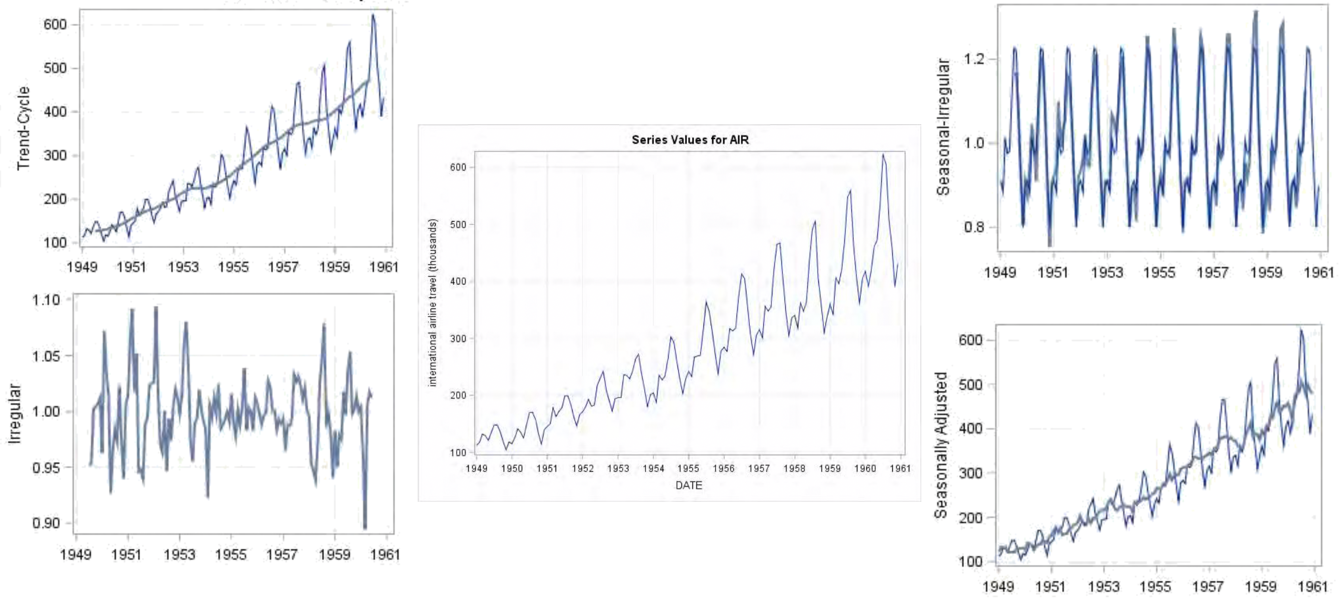
\includegraphics[width=1\textwidth]{trendsaisondecomposition.png}
  \caption{Zeitreihenzerlegung anhand des \enquote{Sashelp.Air} Datensatz. Dieser wurde durch die Komponenten TrendZyklus (Trend-Cycle), Saisonal unregelmäßige (Seasonal-Irregular), Saisonal (Seasonally/Adjusted) und unregelmäßige (Irregular) dargestellt~\cite{Leonard2018}. }
  \label{fig:trendsaisondecomposition}
\end{figure}

Der Informationsgewinn dieser Aufteilung wird durch das Praxisbeispiel aus Abbildung\ \ref{fig:trendsaisondecomposition} deutlich. 
Es werden die internationalen Fluggastdaten aus dem \enquote{Sashelp.Air} Datensatz in einer Zeitreihe dargestellt. Für jeden Monat ist die Gesamtanzahl an grenzüberschreitende Fahrgästen zu sehen. 
Der Datensatz wurde anschließend in:
\begin{itemize}
  \item Trendzyklus Komponente (oben links)
  \item Saisonal unregelmäßige Komponente (oben Rechts)
  \item Unregelmäßige Komponente (unten links)
  \item Saisonale Komponente (unten rechts)
\end{itemize}
aufgeteilt. 
Durch die Trendzyklus Komponente ist ein deutlicher Anstieg zwischen den Jahren 1949 und 1961 erkennbar. 
Die Saisonkomponenten lassen darauf schließen, dass die Anzahl der grenzüberschreitenden Fluggäste stark von den Jahreszeiten abhängen~\cite{Leonard2018}. 

Durch die Zeitreihenzerlegung werden Informationen durch Fokussieren verschiedener Metriken leichter extrahiert. Zudem wird die Komplexität um die jeweiligen Komponenten weiter zu Analysieren stark reduziert. Dennoch ist die Verarbeitung und Visualisierung großer Zeitreihen sehr aufwändig bei dieser Methode.

\subsection{Motivfindung}
Im Gegensatz zu der Zeitreihenzerlegung ist die Idee bei der Motivfindung nicht, die Zeitreihen in Komponenten zu zerlegen, sondern es wird versucht Motive in den Zeitreihen zu identifizieren.
Motive sind nach ihrer Identifizierung verwendbare Merkmale als Eingabe für Lernalgorithmen. Zur Motividentifizierung gibt es unterschiedliche Ansätze:
\begin{itemize}
  \item \enquote{brute-force} basiert
  \item Probabilistische Methoden als Basis
  \item Eine Motivbewertung, welche Motivinstanzen in einer Zielinstanz ausfindig macht
  \item Anomaliedetektion in Teilsequenzen
\end{itemize}

Durch alle diese Ansätze werden die stellen eines Motivs in einer Zeitreihe identifiziert~\cite{Leonard2018}. 
\begin{figure}
  \centering
  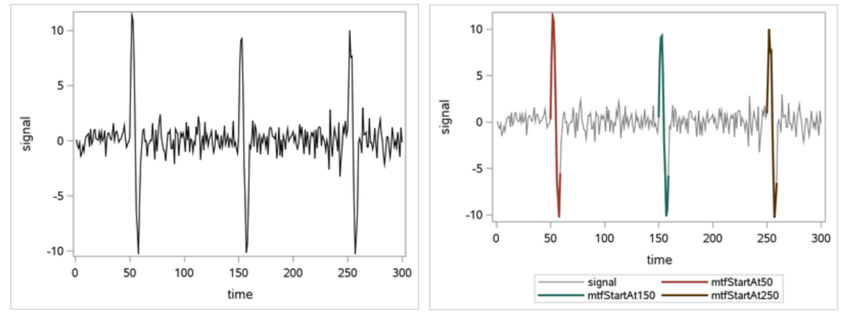
\includegraphics[width=0.8\textwidth]{motifdiscovery.png}
  \caption{Darstellung der in einer Zeitreihe identifizierten Motive~\cite{Leonard2018}. }
  \label{fig:motivdiscovery}
\end{figure}

In Abbildung\ \ref{fig:motivdiscovery} wurde anhand von einem \enquote{brute-force} Ansatz drei Motive in einem Zeitreihendatensatz erkannt.
Je mehr Motive gefunden werden, desto genauer können die Lernalgorithmen die Daten anhand der Motive unterscheiden.
Es wird aber auch komplizierter die Analyse durchzuführen~\cite{Leonard2018}.

Daher ist es auch immer ein Ziel. Die Anzahl an Merkmalen zu reduzieren. 
Um Zeitreihendatensätze zu reduzieren wird die Dimension entstehend durch Parameter oder extrahierten Merkmalen versucht möglichst auf die Notwendigen zu reduzieren. Zeitreihendaten aus Sensoren sind oft hoch korrelierend, was zu einer sehr großen Datenredundanz führt. 
Eine bewerte Technik um Datenmengen aus Sensordaten fester Größe darzustellen ist die \enquote{Fourier Transforamtion}. 

\subsection{Parametrisierung durch die Fourier Transformation}

Bei der Fourier Transformation werden die Signale auf einen Frequenzbereich abgebildet und diese Abbildung mittels Koeffizienten dargestellt. Da es sich bei den kontinuierlichen Sensordaten meist um keinen vollständigen Datenbestand handelt, sondern nur um Datenauszüge, bietet sich die \enquote{Diskrete Fourier Transformation} an.


\begin{equation}
  F_j = \frac{1}{N} \sum_{k=0}^{N-1} f_k W_N^{-kj}  \text{\ \ mit \ \ } W_N = e^{\frac{2\pi i}{N}}
  \label{equ:fourier}
\end{equation}

\begin{equation}
  F_j = \frac{1}{N} (\alpha_0+\alpha_1*e^{i2\pi \frac{t-t_0}{T}}+ \alpha_2*e^{2i2\pi \frac{t-t_0}{T}} + ...)
  \label{equ:fourier}
\end{equation}

Durch die Diskrete Fourier Transformation in Formel\ \ref{equ:fourier} wird der Zeitreihenabschnitt in einer periodische Funktion durch Koeffizienten dargestellt~\cite{Butz2012}. Um die zu analysierenden Merkmale zu reduzieren ist die Idee, dass nicht alle Koeffizienten als Parameter verwenden werden, sondern nur eine Auswahl von diesen. Bekannte Methoden sind dabei entweder die ersten $k$ Koeffizienten zu verwenden. Man speichert quasi nur eine grobe Skizze der Kurven ab. Die ersten Koeffizienten abzuspeichern, behält die tieferen Frequenzen und ist eine sehr naive Herangehensweise. Eine deutlich bessere Methode wäre es die größten Koeffizienten zu verwenden. Diese sind aber sehr aufwändig zu berechnen~\cite{morchen2003time}. Fabian Mörchen stellt dagegen eine Methode in seiner Arbeit \enquote{Time series feature extraction for data mining using DWT and DFT} vor, in der er eine Aggregatsfunktion verwendet, welche die Bedeutung der Koeffizienten misst. Es ist dadurch möglich mit seiner Aggregatsfunktion:

\begin{equation}
  J_k^1(mean(c_j^2), C)
  \label{equ:aggregatefunction}
\end{equation}

eine definierte Menge $k$ an Koeffizienten als Merkmale für Lernalgorithmen als Eingabe zu geben. $k$ entspricht dann der Dimension der zu verarbeitenden Datenmenge. 

\subsection{Extraktion durch Clustern}

Eine weitere Arbeit von Dominique Gay et al. \enquote{Feature Extraction over Multiple Representations for Time Series Calssification} stellt ein Verfahren vor in dem sie Zeitreihendaten so vorverarbeiten, dass in dem Verfahren extrahierte Merkmale die neuen Parameter fester Größe bilden. Dies geschieht in einem Dreischrittverfahren:

\begin{enumerate}
  \item Der Datensatz wird in mehrere Datenrepräsentationen transformiert
  \item Auf jede Repräsentation wird ein Co-Clustering Verfahren angewendet
  \item Aus jeder Repräsentation wird eine Menge an Merkmalen erstellt und daraus ein neuer Datensatz generiert
\end{enumerate}

Für den ersten Schritt schlagen sie verschiedene Transformationsverfahren vor. Beispielsweise Ableitungen oder kumulatives Integrieren. In einem Beispiel sind die Vorteile einer solchen Vorverarbeitung erkennbar. In Abbildung\ \ref{fig:derivative} ist in (a) ein Zweiklassen \enquote{ARSim} Datensatz zu sehen. Dieser ist unverarbeitet und die Klassen sind farblich Markiert. Die Klassen sind in (a) nur sehr schwer separierbar. In (b) wurde der selbe Datensatz durch zweifaches Ableiten transformiert und wieder in einem Datenplot und farblicher Markierung dargestellt. Durch die Transformation sind die Klassen schon deutlicher erkennbar.

\begin{figure}
  \centering
  \includegraphics[width=1\textwidth]{plotAbleitung.png}
  \caption{In (a) ein unverarbeiteter original geplotteter Datensatz und in (b) der gleiche durch zweifache Ableitungen transformierter Datensatz~\cite{Gay2013}.}
  \label{fig:derivative}
\end{figure}

Der transformierte Datensatz bilde somit eine bessere Grundlage um mithilfe von Klassifizierungsalgorithmen die Daten zu Differenzieren. 
Der zweite Schritt ist das Co-Clustering. 
Dabei wird das Clustering als eine Vorverarbeitung für nachfolgende Lernalgorithmen verwendet. 
Die Idee ist es ähnliche Daten zu gruppieren und lokale Muster hervorzuheben~\cite{gay2013feature}. Dabei stellen sie die Kurven in einer Menge $(X,Y)$ dar und fügen jeder dieser Mengen eine Klasse $Cid$ hinzu um sie der jeweiligen Kurve zuzuordnen. Es entsteht eine dreidimensionale Darstellung der Punkte. Das Ganze wird in eine dreidimensionale Gitterstruktur gebracht. Das Endziel ist es Kurven- und Intervallcluster zu erhalten die Anschließend als Merkmalsgrundlage dienen. 

Erreicht wird das durch das Anwenden des \enquote{Khiops Coclustering}\cite{boulle2012functional}. Dabei wird das optimale Gitterfeld durch die Optimierung des Bayes'schen Kriteriums, der sogenannten Kosten ermittelt. 
\begin{equation}
  cost(M) = -log(p(M) \times p(D|M))
  \label{equ:Bayesian}
\end{equation}
Als Resultat lassen sich die Kosten so interpretieren, dass bei niedrigen Kosten eine hohe Kompression der Daten $D$ auf das Modell $M$ herrscht. Wobei das Modell in diesem Fall das optimale Gitterfeld ist.

\begin{figure}
  \centering
  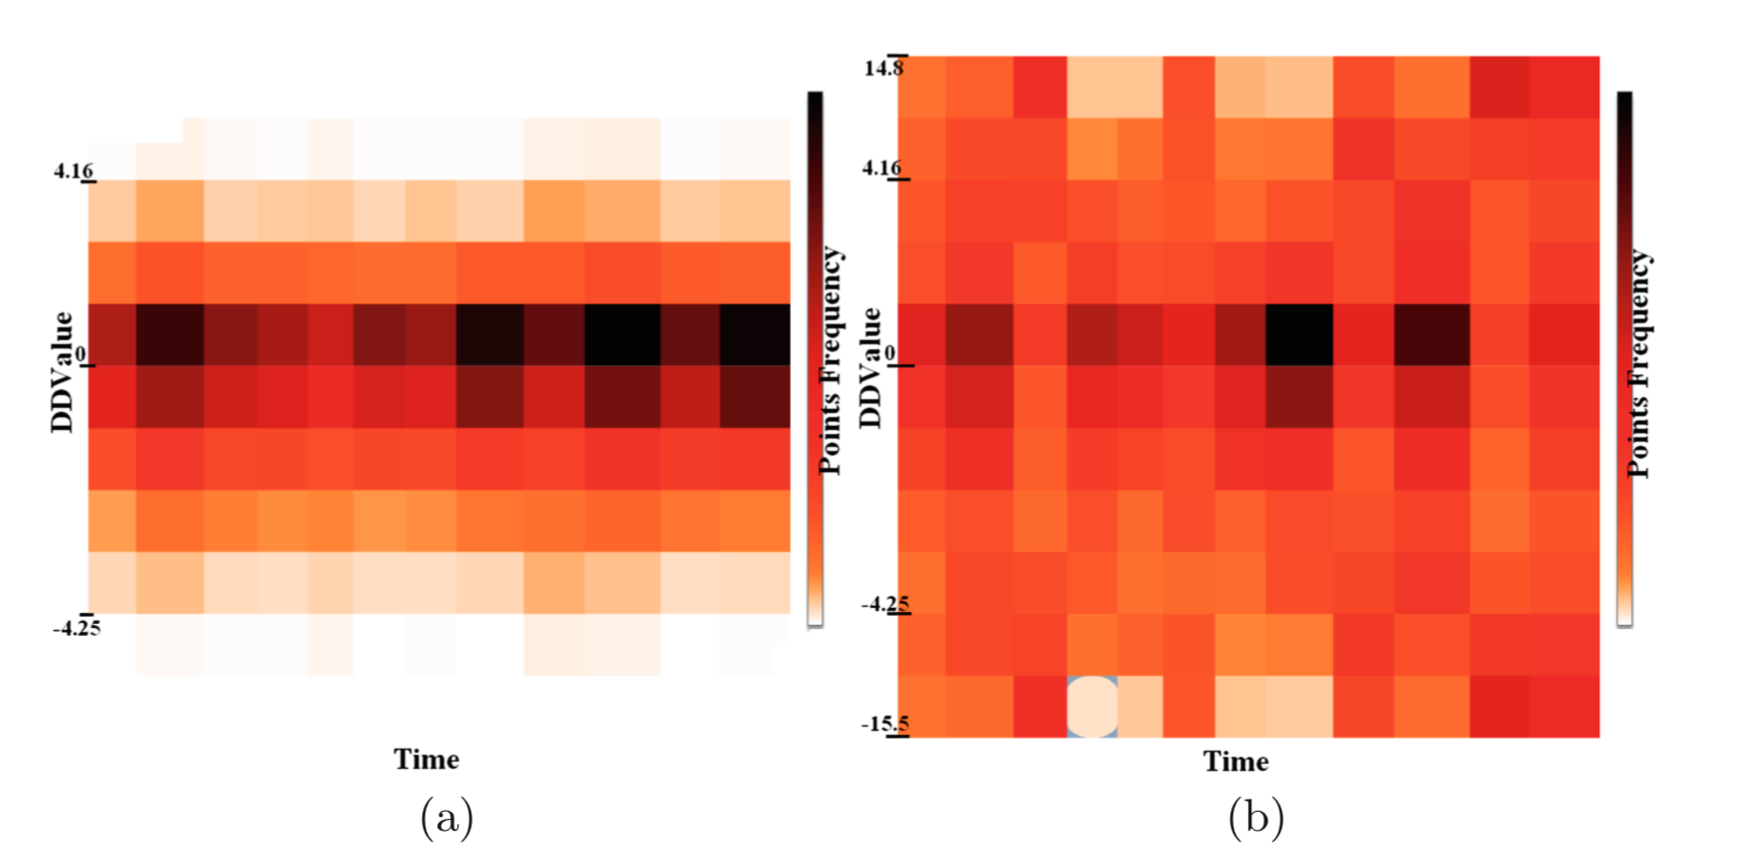
\includegraphics[width=1\textwidth]{coclustering.png}
  \caption{Ergebnis eines Co-Clustering mit \enquote{Khiops Coclustering}~\cite{Gay2013}.}
  \label{fig:coclustering}
\end{figure}

Ein durchgeführtes Co-Clustering ist in Abbildung\ \ref{fig:coclustering} zu sehen. Dabei ist die dritte Dimension Farblich dargestellt. Als Ergebnis sind 25 Cluster von Kurven entstanden. 

Als letzte Schritte müssen noch die Merkmale extrahiert und ein Datensatz generiert werden. Es werden drei Merkmale definiert:

\begin{enumerate}
  \item $K_C$ ein numerisches Merkmal, welches die Unähnlichkeitswahrscheinlichkeit zu allen Kurvenclustern angibt.
  \item Ein kategorisches Merkmal als Index, welcher das nächste Kurvencluster angibt.
  \item $K_Y$ ein numerisches Merkmal, welches die Anzahl an Punkten dieser Kurve in der jeweiligen Klasse angibt.
\end{enumerate}

Durch dieses Verfahren wird die Dimension der Livedaten mit Hilfe von \enquote{Feature Extraktion} auf Drei festgelegt und kann somit durch \enquote{Eager Learning} Algorithmen analysiert werden.

\subsection{Ähnlichkeitsanalyse}
Bei der Ähnlichkeitsanalyse wird der Unterschied unter Berücksichtigung der Ordnung zwischen Eingabe- und Zielsequenz gemessen. 
Zusätzlich können diese Verfahren auch die Zielsequenz in Richtung der Eingabesequenz verschieben um möglichst effizient die Ähnlichkeit zu messen~\cite{Leonard2018}. 
In Abbildung\ \ref{fig:similarityanalysis} ist eine solche Verschiebung durch ein Ähnlichkeitsmaß abgebildet. 
Dabei wird die Zielsequenz im oberen rechten Bild auf die Eingabesequenz im oberen linken Bild verschoben. Die Verschiebung und Ähnlichkeit ist in dem Bild unten Rechts dargestellt.
\begin{figure}
  \centering
  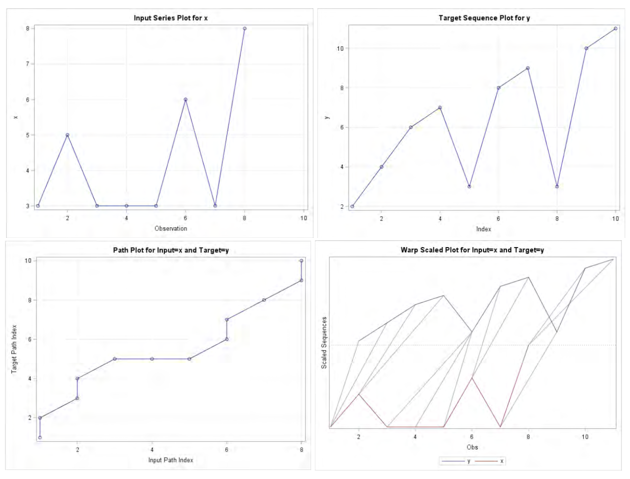
\includegraphics[width=0.8\textwidth]{similarityanalysis.png}
  \caption{Darstellung einer Ähnlichkeitsanalyse auf Basis einer Datenverschiebung. Oben links die Eingangssequenz wird wie in der Abbildung unten rechts auf die Zielsequenz oben rechts verschoben~\cite{Leonard2018}.}
  \label{fig:similarityanalysis}
\end{figure}

Dieses Ähnlichkeitsmaß stellt ein Merkmal da anhand dessen Sensordaten in Form von Zeitreihendaten verglichen werden können. 
Durch die Ähnlichkeitsanalyse können auch mehrere Sequenzen miteinander verglichen werden und daraus eine Ähnlichkeitsmatrix erstellt werden.
\section{Zusammenfassung}


%%%%%%%%%%%%%%%%%%%%%%%%%%%%%%%%%%%%%%%%%%%%%%%%%%%%%%%%%%%%%%%%%%%%%%%%%%%%%%%

\bibliographystyle{splncs03}
\bibliography{paper}
%%\nocite{*}
Alle Links wurden zuletzt am 10.12.2018 geprüft.
\end{document}
